\section*{Procedimentos}
% ---------- estilos dos diagramas (podem ficar no preâmbulo) ----------
\tikzset{
  etapa/.style={draw, rounded corners=2pt, fill=blue!6, align=center,
                text width=5.6cm, minimum height=0.9cm, font=\small},
  io/.style={align=flush left, text width=5.2cm, font=\footnotesize},
  seta/.style={-{Stealth[length=2mm]}, thick},
  setaio/.style={-{Stealth[length=1.6mm]}, gray!70!black},
  titulo/.style={font=\footnotesize\bfseries, text=gray!60!black},
}


\subsection*{Método dos perfis delgados}

O procedimento seguido está esquematizado na Figura~\ref{fig:diag_thin} e foi
implementado em MATLAB. Cada etapa indica as entradas (à esquerda) e as saídas
(à direita).

\begin{figure}[H]
\centering
\begin{tikzpicture}[node distance=0.45cm]
  % etapas
  \node[etapa] (e1) {\textbf{1.} Importação da geometria};
  \node[etapa, below=of e1] (e2) {\textbf{2.} Interpolação e linha média};
  \node[etapa, below=of e2] (e3) {\textbf{3.} Declive da linha média};
  \node[etapa, below=of e3] (e4) {\textbf{4.} Mudança de variável $x \rightarrow \theta$};
  \node[etapa, below=of e4] (e5) {\textbf{5.} Coeficientes de Fourier};
  \node[etapa, below=of e5] (e6) {\textbf{6.} Coeficientes aerodinâmicos};
  \node[etapa, below=of e6] (e7) {\textbf{7.} Estudo de convergência em $N$};
  \foreach \a/\b in {e1/e2,e2/e3,e3/e4,e4/e5,e5/e6,e6/e7}
    \draw[seta] (\a) -- (\b);
  % entradas
  \node[io, left=0.5cm of e1, align=flush right] (i1) {Ficheiro de coordenadas (formato Lednicer): 36 pontos no extradorso e 36 no intradorso};
  \node[io, left=0.5cm of e2, align=flush right] (i2) {$(x_u,z_u)$, $(x_l,z_l)$; $N = 1000$ pontos};
  \node[io, left=0.5cm of e3, align=flush right] (i3) {$z_c(x)$};
  \node[io, left=0.5cm of e4, align=flush right] (i4) {$dz_c/dx\,(x)$; $x = \tfrac{1}{2}(1-\cos\theta)$};
  \node[io, left=0.5cm of e5, align=flush right] (i5) {$dz_c/dx\,(\theta)$, $\theta \in [0,\pi]$};
  \node[io, left=0.5cm of e6, align=flush right] (i6) {$I_0$, $A_1$; $\alpha \in [-20^\circ, 20^\circ]$, passo $0{,}5^\circ$};
  \node[io, left=0.5cm of e7, align=flush right] (i7) {$N \in \{50,\dots,10\,000\}$; tolerâncias $\Delta c_l = 10^{-3}$, $\Delta\alpha_{L=0} = 0{,}01^\circ$};
  % saídas
  \node[io, right=0.5cm of e1] (o1) {$(x_u,z_u)$, $(x_l,z_l)$, normalizados pela corda};
  \node[io, right=0.5cm of e2] (o2) {$z_c = \tfrac{1}{2}(z_u+z_l)$; espessura $z_u - z_l$};
  \node[io, right=0.5cm of e3] (o3) {$dz_c/dx\,(x)$};
  \node[io, right=0.5cm of e4] (o4) {$dz_c/dx\,(\theta)$};
  \node[io, right=0.5cm of e5] (o5) {$I_0$, $A_1$ (regra dos trapézios)};
  \node[io, right=0.5cm of e6] (o6) {$\alpha_{L=0}$, $c_l(\alpha)$, $dc_l/d\alpha = 2\pi$};
  \node[io, right=0.5cm of e7] (o7) {$N$ que cumpre as tolerâncias; erros de $c_l(5^\circ)$ e $\alpha_{L=0}$};
  \foreach \k in {1,...,7} {
    \draw[setaio] (i\k) -- (e\k);
    \draw[setaio] (e\k) -- (o\k);
  }
  \path (e1.north) ++(0,0.6) coordinate (topo);
  \node[titulo] at (i1 |- topo) {Entradas};
  \node[titulo] at (o1 |- topo) {Saídas};
\end{tikzpicture}
\caption{Diagrama de blocos do método dos perfis delgados.}
\label{fig:diag_thin}
\end{figure}

\noindent\textbf{1. Importação da geometria.} As coordenadas do perfil são lidas do
ficheiro da base de dados da UIUC (formato Lednicer), com 36 pontos em cada
superfície, já normalizados pela corda.

\noindent\textbf{2. Interpolação e linha média.} As duas superfícies são interpoladas em
$N$ pontos igualmente espaçados em $x/c$, usando interpolação \emph{pchip} na
variável $\sqrt{x}$, que acompanha melhor a variação de $z$ junto ao bordo de
ataque. A linha média e a espessura obtêm-se por
\[
  z_c(x) = \frac{z_u(x) + z_l(x)}{2}, \qquad t(x) = z_u(x) - z_l(x),
\]
o que corresponde a medir a meia-distância na vertical e não na perpendicular à
linha média, uma aproximação válida para perfis finos. A Figura~\ref{fig:geom}
mostra o perfil e a sua linha média.

\begin{figure}[H]
  \centering
  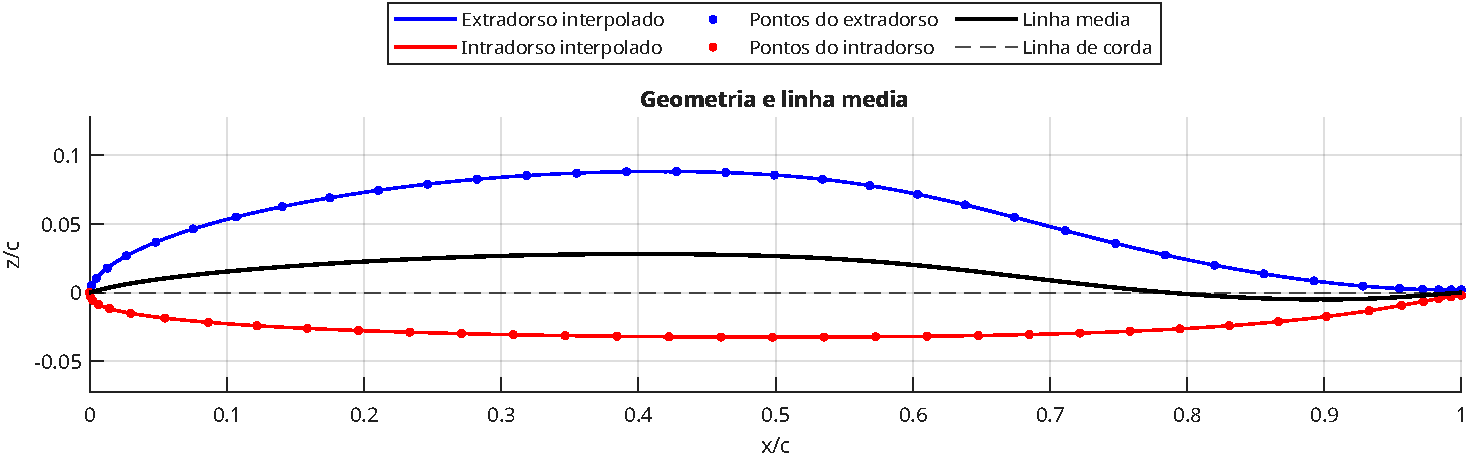
\includegraphics[width=0.85\textwidth]{imagens/geometry.pdf}
  \caption{Perfil Roncz/Marske-7 e respetiva linha média.}
  \label{fig:geom}
\end{figure}

\noindent\textbf{3. Declive da linha média.} O declive $dz_c/dx$ calcula-se por diferenças
finitas centradas (função \texttt{gradient}).

\noindent\textbf{4. Mudança de variável.} A teoria dos perfis delgados exprime os integrais
na variável $\theta$, definida por
\[
  x = \frac{c}{2}\,(1 - \cos\theta), \qquad 0 \le \theta \le \pi ,
\]
pelo que o declive é reinterpolado numa malha uniforme em $\theta$.

\noindent\textbf{5. Coeficientes de Fourier.} Os integrais
\[
  I_0 = \frac{1}{\pi}\int_0^{\pi} \frac{dz_c}{dx}\,d\theta, \qquad
  A_1 = \frac{2}{\pi}\int_0^{\pi} \frac{dz_c}{dx}\cos\theta\,d\theta
\]
calculam-se numericamente pela regra dos trapézios, sendo $A_0 = \alpha - I_0$.

\noindent\textbf{6. Coeficientes aerodinâmicos.} O coeficiente de sustentação e o ângulo de
sustentação nula são dados por
\[
  c_l = 2\pi\left(A_0 + \frac{A_1}{2}\right) = 2\pi\,(\alpha - \alpha_{L=0}),
  \qquad
  \alpha_{L=0} = I_0 - \frac{A_1}{2},
\]
para $\alpha$ entre $-20^\circ$ e $20^\circ$ com incrementos de $0{,}5^\circ$. O
declive da curva de sustentação é $dc_l/d\alpha = 2\pi$~rad$^{-1}$,
independente da geometria.

\noindent\textbf{7. Estudo de convergência.} Repete-se o cálculo para
$N$ entre $50$ e $10\,000$ e comparam-se $c_l(5^\circ)$ e $\alpha_{L=0}$ com os
valores obtidos para o maior $N$. Com $N = 1000$, os erros são inferiores às
tolerâncias impostas ($10^{-3}$ em $c_l$ e $0{,}01^\circ$ em $\alpha_{L=0}$).


\subsection*{Método dos painéis}

Utilizou-se o método dos painéis de vórtices com intensidade linear
{ref: Katz \& Plotkin}, implementado em MATLAB e esquematizado na
Figura~\ref{fig:diag_paineis}.

\begin{figure}[H]
\centering
\begin{tikzpicture}[node distance=0.45cm]
  \node[etapa] (p1) {\textbf{1.} Painelização do perfil};
  \node[etapa, below=of p1] (p2) {\textbf{2.} Coeficientes de influência};
  \node[etapa, below=of p2] (p3) {\textbf{3.} Condições de fronteira};
  \node[etapa, below=of p3] (p4) {\textbf{4.} Resolução do sistema linear};
  \node[etapa, below=of p4] (p5) {\textbf{5.} Velocidade tangencial e $C_p$};
  \node[etapa, below=of p5] (p6) {\textbf{6.} Coeficientes de força};
  \node[etapa, below=of p6] (p7) {\textbf{7.} Pós-processamento};
  \foreach \a/\b in {p1/p2,p2/p3,p3/p4,p4/p5,p5/p6,p6/p7}
    \draw[seta] (\a) -- (\b);
  % ciclo de convergência
  \draw[seta, dashed] (p6.east) -- ++(0.3,0) |- (p1.east);
  % entradas
  \node[io, left=0.5cm of p1, align=flush right] (j1) {Ficheiro de coordenadas; número de painéis $N$};
  \node[io, left=0.5cm of p2, align=flush right] (j2) {Nós $(x_j,z_j)$; pontos de controlo $(x_i,z_i)$};
  \node[io, left=0.5cm of p3, align=flush right] (j3) {$V_\infty$, $\alpha$; normais $\mathbf{n}_i$};
  \node[io, left=0.5cm of p4, align=flush right] (j4) {Matriz $\mathbf{A}$, vetor $\mathbf{b}$};
  \node[io, left=0.5cm of p5, align=flush right] (j5) {$\gamma_j$; influências; tangentes $\mathbf{t}_i$};
  \node[io, left=0.5cm of p6, align=flush right] (j6) {$C_{p,i}$, $\mathbf{n}_i$, $\Delta s_i$, $\alpha$};
  \node[io, left=0.5cm of p7, align=flush right] (j7) {$\gamma_j$, $V_{t,i}$, $C_{p,i}$; malha de pontos em redor do perfil};
  % saídas
  \node[io, right=0.75cm of p1] (q1) {Nós, pontos de controlo, $\mathbf{t}_i$, $\mathbf{n}_i$, $\Delta s_i$};
  \node[io, right=0.75cm of p2] (q2) {Matriz $\mathbf{A}$, $(N{+}1)\times(N{+}1)$};
  \node[io, right=0.75cm of p3] (q3) {Vetor $\mathbf{b}$; condição de Kutta $\gamma_1 + \gamma_{N+1} = 0$};
  \node[io, right=0.75cm of p4] (q4) {Intensidades $\gamma_j$ nos $N+1$ nós};
  \node[io, right=0.75cm of p5] (q5) {$V_{t,i}$, $C_{p,i}$; verificação $V_{n,i} \approx 0$};
  \node[io, right=0.75cm of p6] (q6) {$C_x$, $C_z$ $\rightarrow$ $c_l$, $c_{d,p}$; ciclo em $N$ até variação de $c_l(5^\circ) < 0{,}5\,\%$};
  \node[io, right=0.75cm of p7] (q7) {Linhas de corrente, ponto de estagnação, $C_{p,\min}$};
  \foreach \k in {1,...,7} {
    \draw[setaio] (j\k) -- (p\k);
    \draw[setaio] (p\k) -- (q\k);
  }
  \path (p1.north) ++(0,0.6) coordinate (topo);
  \node[titulo] at (j1 |- topo) {Entradas};
  \node[titulo] at (q1 |- topo) {Saídas};
\end{tikzpicture}
\caption{Diagrama de blocos do método dos painéis. A seta a tracejado
representa o estudo de convergência em $N$.}
\label{fig:diag_paineis}
\end{figure}

\noindent\textbf{1. Painelização.} O contorno do perfil é percorrido no sentido
anti-horário, do bordo de fuga pelo extradorso até ao bordo de ataque e
regressando pelo intradorso. Cada superfície é reinterpolada (\emph{pchip}) em
$N/2$ painéis de igual comprimento de arco. Para cada painel calculam-se o ponto
de controlo (ponto médio), o comprimento $\Delta s_i$ e os vetores unitários
tangente $\mathbf{t}_i$ e normal exterior $\mathbf{n}_i$.

\noindent\textbf{2. Coeficientes de influência.} Em cada painel $j$ a intensidade dos
vórtices varia linearmente entre os valores nodais $\gamma_j$ e $\gamma_{j+1}$.
A velocidade induzida por um painel num ponto de controlo $i$ calcula-se
analiticamente num referencial local alinhado com o painel e é depois rodada para
o referencial global. Os coeficientes $a_{ij}$ correspondem à componente normal
dessa velocidade para intensidade unitária em cada nó.

\noindent\textbf{3. Condições de fronteira.} Impõe-se que a velocidade normal seja nula em
cada ponto de controlo (impermeabilidade),
\[
  \sum_{j=1}^{N+1} a_{ij}\,\gamma_j = -\mathbf{V}_\infty \cdot \mathbf{n}_i ,
  \qquad i = 1,\dots,N ,
\]
o que dá $N$ equações para $N+1$ incógnitas. A equação que falta é a condição de
Kutta, que impõe intensidade nula no bordo de fuga:
$\gamma_1 + \gamma_{N+1} = 0$. Como o perfil tem bordo de fuga com espessura
finita, esta condição é aplicada de forma aproximada.

\noindent\textbf{4. Resolução do sistema.} O sistema
$\mathbf{A}\,\boldsymbol{\gamma} = \mathbf{b}$ resolve-se diretamente
(operador \texttt{\textbackslash} do MATLAB).

\noindent\textbf{5. Velocidade tangencial e coeficiente de pressão.} Em cada ponto de
controlo soma-se a velocidade do escoamento livre com a induzida por todos os
painéis. A componente tangencial dá o coeficiente de pressão,
\[
  C_{p,i} = 1 - \left(\frac{V_{t,i}}{V_\infty}\right)^2 ,
\]
e a componente normal $V_{n,i}$, que deve ser nula, serve para verificar a
solução.

\noindent\textbf{6. Coeficientes de força.} Integrando a pressão ao longo do contorno,
\[
  C_x = -\sum_i C_{p,i}\, n_{x,i}\,\Delta s_i , \qquad
  C_z = -\sum_i C_{p,i}\, n_{z,i}\,\Delta s_i ,
\]
e projetando nas direções perpendicular e paralela ao escoamento livre,
\[
  c_l = -C_x \sin\alpha + C_z \cos\alpha , \qquad
  c_{d,p} = C_x \cos\alpha + C_z \sin\alpha .
\]
Repete-se o cálculo para $N$ entre $20$ e $800$ painéis a $\alpha = 5^\circ$
(seta a tracejado na Figura~\ref{fig:diag_paineis}); escolheu-se $N = 260$, a
partir do qual o erro de $c_l$ em relação a $N = 800$ é inferior a $0{,}5\,\%$.

\noindent\textbf{7. Pós-processamento.} Com as intensidades $\gamma_j$ calcula-se a
velocidade numa malha de pontos em redor do perfil para traçar as linhas de
corrente. O ponto de estagnação localiza-se onde $V_t$ muda de sinal junto ao
bordo de ataque (interpolação linear), e regista-se o $C_p$ mínimo e a sua
posição.
